

\tikzset{every picture/.style={line width=0.75pt}} %set default line width to 0.75pt        

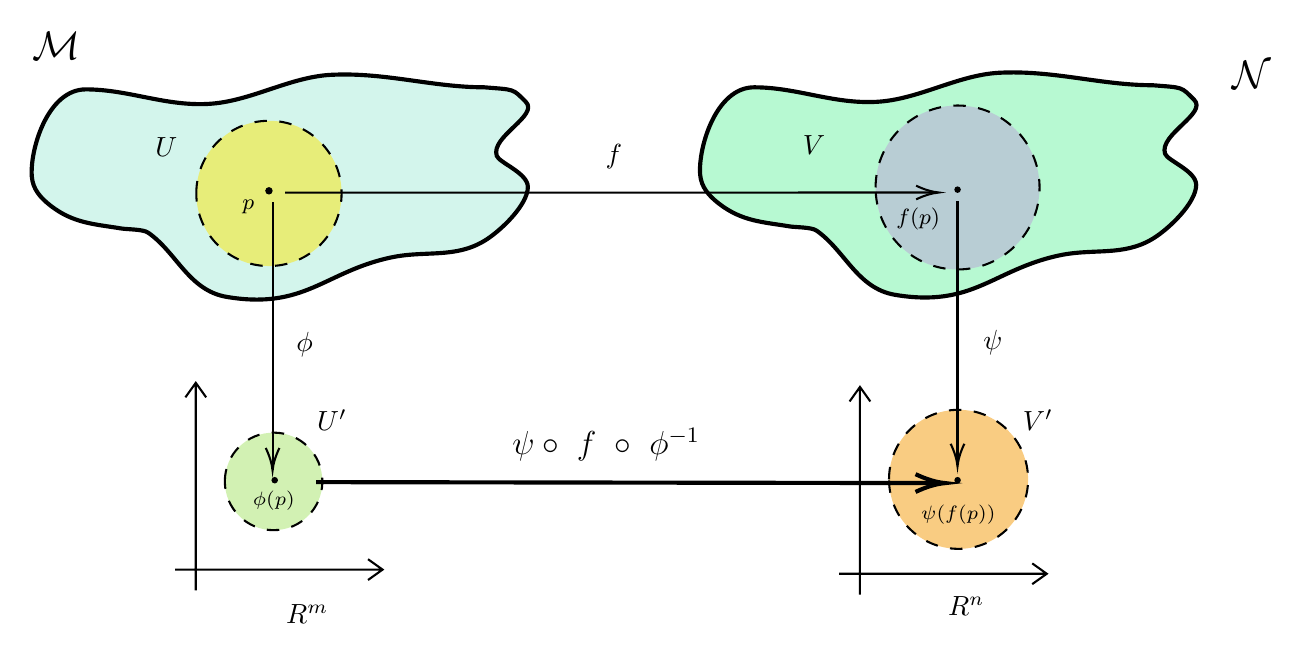
\begin{tikzpicture}[x=0.75pt,y=0.75pt,yscale=-1,xscale=1]
%uncomment if require: \path (0,351); %set diagram left start at 0, and has height of 351

%Shape: Circle [id:dp4604718091966047] 
\draw  [fill={rgb, 255:red, 184; green, 233; blue, 134 }  ,fill opacity=0.63 ][dash pattern={on 4.5pt off 4.5pt}] (119,224.5) .. controls (119,211.52) and (129.52,201) .. (142.5,201) .. controls (155.48,201) and (166,211.52) .. (166,224.5) .. controls (166,237.48) and (155.48,248) .. (142.5,248) .. controls (129.52,248) and (119,237.48) .. (119,224.5) -- cycle ;
%Shape: Circle [id:dp3442356821329243] 
\draw  [fill={rgb, 255:red, 245; green, 166; blue, 35 }  ,fill opacity=0.57 ][dash pattern={on 4.5pt off 4.5pt}] (439,223.5) .. controls (439,205) and (454,190) .. (472.5,190) .. controls (491,190) and (506,205) .. (506,223.5) .. controls (506,242) and (491,257) .. (472.5,257) .. controls (454,257) and (439,242) .. (439,223.5) -- cycle ;
%Curve Lines [id:da8514602322717827] 
\draw [fill={rgb, 255:red, 8; green, 233; blue, 99 }  ,fill opacity=0.29 ][line width=1.5] [line join = round][line cap = round]   (566,33.63) .. controls (541.07,33.63) and (518.02,26.24) .. (492,27.63) .. controls (471.94,28.71) and (453.25,40.57) .. (433,41.63) .. controls (411.98,42.74) and (394.57,34.63) .. (374,34.63) .. controls (355.59,34.63) and (347.01,63.73) .. (348,76.63) .. controls (348.47,82.7) and (352.18,86.88) .. (357,90.63) .. controls (368.08,99.25) and (378.24,99.51) .. (391,101.63) .. controls (393.95,102.13) and (401.58,101.96) .. (404,103.63) .. controls (417.88,113.24) and (423.56,131.56) .. (442,134.63) .. controls (479.55,140.89) and (489.14,122.46) .. (521,115.63) .. controls (537.52,112.09) and (551.69,116.22) .. (566,107.63) .. controls (573.71,103.01) and (587,90.32) .. (587,81.63) .. controls (587,74.9) and (573.1,69.94) .. (572,66.63) .. controls (568.91,57.36) and (592.59,47.22) .. (586,40.63) .. controls (579.54,34.17) and (581,34.85) .. (566,33.63) -- cycle ;
%Curve Lines [id:da2024130737434997] 
\draw [fill={rgb, 255:red, 211; green, 245; blue, 236 }  ,fill opacity=1 ][line width=1.5] [line join = round][line cap = round]   (244,34.63) .. controls (219.07,34.63) and (196.02,27.24) .. (170,28.63) .. controls (149.94,29.71) and (131.25,41.57) .. (111,42.63) .. controls (89.98,43.74) and (72.57,35.63) .. (52,35.63) .. controls (33.59,35.63) and (25.01,64.73) .. (26,77.63) .. controls (26.47,83.7) and (30.18,87.88) .. (35,91.63) .. controls (46.08,100.25) and (56.24,100.51) .. (69,102.63) .. controls (71.95,103.13) and (79.58,102.96) .. (82,104.63) .. controls (95.88,114.24) and (101.56,132.56) .. (120,135.63) .. controls (157.55,141.89) and (167.14,123.46) .. (199,116.63) .. controls (215.52,113.09) and (229.69,117.22) .. (244,108.63) .. controls (251.71,104.01) and (265,91.32) .. (265,82.63) .. controls (265,75.9) and (251.1,70.94) .. (250,67.63) .. controls (246.91,58.36) and (270.59,48.22) .. (264,41.63) .. controls (257.54,35.17) and (259,35.85) .. (244,34.63) -- cycle ;
%Shape: Circle [id:dp06624735745121968] 
\draw  [fill={rgb, 255:red, 248; green, 231; blue, 28 }  ,fill opacity=0.55 ][dash pattern={on 4.5pt off 4.5pt}] (105.25,85.75) .. controls (105.25,66.42) and (120.92,50.75) .. (140.25,50.75) .. controls (159.58,50.75) and (175.25,66.42) .. (175.25,85.75) .. controls (175.25,105.08) and (159.58,120.75) .. (140.25,120.75) .. controls (120.92,120.75) and (105.25,105.08) .. (105.25,85.75) -- cycle ;
%Shape: Circle [id:dp05380630291243382] 
\draw  [fill={rgb, 255:red, 189; green, 16; blue, 224 }  ,fill opacity=0.19 ][dash pattern={on 4.5pt off 4.5pt}] (432.53,82.9) .. controls (432.53,61.08) and (450.22,43.4) .. (472.03,43.4) .. controls (493.85,43.4) and (511.53,61.08) .. (511.53,82.9) .. controls (511.53,104.72) and (493.85,122.4) .. (472.03,122.4) .. controls (450.22,122.4) and (432.53,104.72) .. (432.53,82.9) -- cycle ;
%Straight Lines [id:da795651220900737] 
\draw    (142,90.08) -- (142,217.32) ;
\draw [shift={(142,219.32)}, rotate = 270] [color={rgb, 255:red, 0; green, 0; blue, 0 }  ][line width=0.75]    (10.93,-3.29) .. controls (6.95,-1.4) and (3.31,-0.3) .. (0,0) .. controls (3.31,0.3) and (6.95,1.4) .. (10.93,3.29)   ;
%Straight Lines [id:da47228720125648727] 
\draw    (472,89.32) -- (472,215.32) ;
\draw [shift={(472,217.32)}, rotate = 270] [color={rgb, 255:red, 0; green, 0; blue, 0 }  ][line width=0.75]    (10.93,-3.29) .. controls (6.95,-1.4) and (3.31,-0.3) .. (0,0) .. controls (3.31,0.3) and (6.95,1.4) .. (10.93,3.29)   ;
%Shape: Axis 2D [id:dp4084611261773249] 
\draw  (95,267) -- (195,267)(105,177) -- (105,277) (188,262) -- (195,267) -- (188,272) (100,184) -- (105,177) -- (110,184)  ;
%Shape: Axis 2D [id:dp12556457670089383] 
\draw  (415,269) -- (515,269)(425,179) -- (425,279) (508,264) -- (515,269) -- (508,274) (420,186) -- (425,179) -- (430,186)  ;
%Straight Lines [id:da43480740287261954] 
\draw [line width=1.5]    (463,225.31) -- (163,224.85) ;
\draw [shift={(466,225.32)}, rotate = 180.09] [color={rgb, 255:red, 0; green, 0; blue, 0 }  ][line width=1.5]    (14.21,-4.28) .. controls (9.04,-1.82) and (4.3,-0.39) .. (0,0) .. controls (4.3,0.39) and (9.04,1.82) .. (14.21,4.28)   ;
%Shape: Circle [id:dp17641131819546774] 
\draw  [fill={rgb, 255:red, 0; green, 0; blue, 0 }  ,fill opacity=1 ] (139,84.5) .. controls (139,83.81) and (139.56,83.25) .. (140.25,83.25) .. controls (140.94,83.25) and (141.5,83.81) .. (141.5,84.5) .. controls (141.5,85.19) and (140.94,85.75) .. (140.25,85.75) .. controls (139.56,85.75) and (139,85.19) .. (139,84.5) -- cycle ;
%Shape: Circle [id:dp9098380916442051] 
\draw  [fill={rgb, 255:red, 0; green, 0; blue, 0 }  ,fill opacity=1 ] (142,223.93) .. controls (142,224.5) and (142.46,224.97) .. (143.03,224.97) .. controls (143.6,224.97) and (144.07,224.5) .. (144.07,223.93) .. controls (144.07,223.36) and (143.6,222.9) .. (143.03,222.9) .. controls (142.46,222.9) and (142,223.36) .. (142,223.93) -- cycle ;
%Straight Lines [id:da12001174564982175] 
\draw    (148,85.37) -- (461,85.32) ;
\draw [shift={(463,85.32)}, rotate = 179.99] [color={rgb, 255:red, 0; green, 0; blue, 0 }  ][line width=0.75]    (10.93,-3.29) .. controls (6.95,-1.4) and (3.31,-0.3) .. (0,0) .. controls (3.31,0.3) and (6.95,1.4) .. (10.93,3.29)   ;
%Shape: Circle [id:dp6218977499267407] 
\draw  [fill={rgb, 255:red, 0; green, 0; blue, 0 }  ,fill opacity=1 ] (471,83.93) .. controls (471,84.5) and (471.46,84.97) .. (472.03,84.97) .. controls (472.6,84.97) and (473.07,84.5) .. (473.07,83.93) .. controls (473.07,83.36) and (472.6,82.9) .. (472.03,82.9) .. controls (471.46,82.9) and (471,83.36) .. (471,83.93) -- cycle ;
%Shape: Circle [id:dp25390351977169645] 
\draw  [fill={rgb, 255:red, 0; green, 0; blue, 0 }  ,fill opacity=1 ] (471,223.93) .. controls (471,224.5) and (471.46,224.97) .. (472.03,224.97) .. controls (472.6,224.97) and (473.07,224.5) .. (473.07,223.93) .. controls (473.07,223.36) and (472.6,222.9) .. (472.03,222.9) .. controls (471.46,222.9) and (471,223.36) .. (471,223.93) -- cycle ;

% Text Node
\draw (84,57.4) node [anchor=north west][inner sep=0.75pt]    {$U$};
% Text Node
\draw (147,282.4) node [anchor=north west][inner sep=0.75pt]    {$\mathbb{R}^{m}$};
% Text Node
\draw (466,278.4) node [anchor=north west][inner sep=0.75pt]    {$\mathbb{R}^{n}$};
% Text Node
\draw (162,188.4) node [anchor=north west][inner sep=0.75pt]    {$U '$};
% Text Node
\draw (502,188.4) node [anchor=north west][inner sep=0.75pt]    {$V'$};
% Text Node
\draw (152,151.4) node [anchor=north west][inner sep=0.75pt]    {$\phi $};
% Text Node
\draw (453,234.4) node [anchor=north west][inner sep=0.75pt]  [font=\scriptsize]  {$\psi ( f( p))$};
% Text Node
\draw (256,197.4) node [anchor=north west][inner sep=0.75pt]  [font=\large]  {$\psi \circ \ f\ \circ \ \phi ^{-1}$};
% Text Node
\draw (25,6.4) node [anchor=north west][inner sep=0.75pt]  [font=\Large]  {$\mathcal{M}$};
% Text Node
\draw (396,56.4) node [anchor=north west][inner sep=0.75pt]    {$V$};
% Text Node
\draw (126,87.4) node [anchor=north west][inner sep=0.75pt]  [font=\footnotesize]  {$p$};
% Text Node
\draw (131,227.4) node [anchor=north west][inner sep=0.75pt]  [font=\scriptsize]  {$\phi ( p)$};
% Text Node
\draw (441,91.4) node [anchor=north west][inner sep=0.75pt]  [font=\footnotesize]  {$f( p)$};
% Text Node
\draw (603,20.4) node [anchor=north west][inner sep=0.75pt]  [font=\Large]  {$\mathcal{N}$};
% Text Node
\draw (483,150.4) node [anchor=north west][inner sep=0.75pt]    {$\psi $};
% Text Node
\draw (301,60.4) node [anchor=north west][inner sep=0.75pt]    {$f$};


\end{tikzpicture}
